% Context and motivation
Natural language processing methods for the generation of symbolic music have experienced significant advancements in recent years.
The transformer architecture, first introduced on text by Vaswani et al. in 2017\cite{vaswani_attention_2017}, has been later used to generate scores for various instruments, in diverse styles and genres\cite{le_natural_2024}.
% REORGANIZE
A user study conducted by Bacot et al.\cite{bacot_tablature_2025} showed a potential need for accompaniment generation tools for guitarists.
The questionnaire was answered by 31 guitarist-composers, and 7 of them followed up with an interview.
During the interviews, several guitarists answered that they would like to be able to generate bass guitar lines and drum parts without requiring familiarity with the instruments.
Indeed, guitarists often resort to writing basic bass lines to accompany their compositions, and an AI tool could perform this functional task for them.

% Objectives
This need is the starting point for this project, proposed by the Algomus team, part of the CRIStAL laboratory.
We focus on the conditional aspect of symbolic music generation, for an instrument that has not been thoroughly studied yet: the bass guitar.
Specifically, the goal is to generate bass guitar tablatures given other instruments' scores, in the context of Western popular music.
Our objective is to try several combinations of conditioning instruments and to evaluate the quality of the generated tablatures both numerically and with the help of musicians.


% Terms definition (tablature, add the period when it was used)
% Difference between guitar and bass (role in the music)
To better understand what is at stake in this challenge, we will begin by precisely defining the terms of the subject and the role of the bass guitar in the context of Western popular music.
Since the human ear perceives low-frequency pulses more distinctly, the bass guitar is considered part of the rhythmic section of the band (together with the drums)\cite{hove_superior_2014}.
However, the bass guitar also performs a harmonic — and sometimes melodic — role in the music, sustaining the lead instruments and adding groove to the composition.
Its adaptability makes the bass guitar a crucial component across various genres of Western popular music.


Historically, tablatures have been used since the Renaissance period as a simplified notation system for string instruments like the lute.
Originating around the 16th century, tablatures were an intuitive alternative to staff notation, allowing musicians to bypass the complexity of interpreting pitches.
This system explicitly linked symbols to physical actions on the instrument, such as pressing specific frets or strings.
In the 20th century, and with the rise of internet forums and music sharing platforms, tablatures became a popular way to share music scores among amateur musicians.
First in ASCII format, tablatures were later digitalized and standardized in formats like GuitarPro (GP), further extending their use for learning, practice, and composition in genres ranging from classical to popular music\cite{sarmento_dadagp_2021}.
Tablatures originally did not contain rhythmic information, which is why they are generally combined with scores.
As a majority of guitarists learn many aspects of the songs they play by listening to them\cite{green_how_2001},
tablatures are more of a prescriptive way to teach how to play a song that is already known by the musician.
Tablatures are part of what is called symbolic music, distinguished from audio music.
This project focuses on symbolic music, which corresponds to the written representation of music.
This representation can be in the form of scores or tablatures, but no audio will be involved in the generation process.


% FUNKO JAZZ, LENNY TRAVITZ, JACO PASTORIUS, VULFPECK
% add a fig Time is running out, melodic and rhythmic bass
\begin{figure}[!ht]
    \centering
    \begin{minipage}{0.45\textwidth}
        \centering
        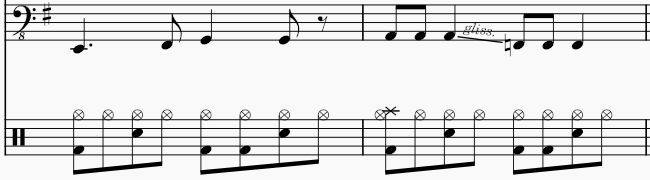
\includegraphics[width=.99\linewidth]{../images-figures/rhythmic_tab_karma_police.png}
    \end{minipage}%
    \hfill
    \begin{minipage}{0.45\textwidth}
        \centering
        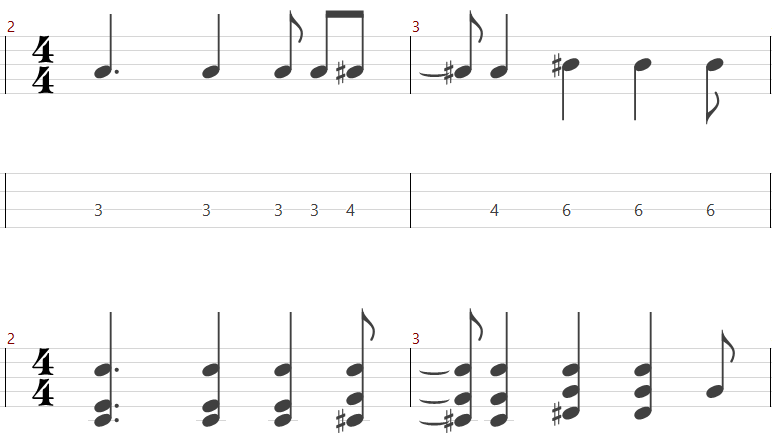
\includegraphics[width=.7\linewidth]{../images-figures/melodic_tab_eiirp.png}
    \end{minipage}
    \caption{Rhythmic (left) and melodic (right) extracts in Karma Police (left) and Everything in its Right Place (right) by Radiohead.}
    \label{fig:bass_tab_TIRO}
\end{figure}


Figure~\ref{fig:bass_tab_TIRO} shows a score extract of both a rhythmic and a melodic bass.
In the extract on the left, the bass guitar plays a rhythmic role, accompanying the drums in its pulsating rhythm 
whereas on the right, the bass guitar plays a melodic role, following the lead guitar's melody at a lower pitch.
In both these extracts, the bass guitar is essential to the song's structure.
It adds grooves, harmonies and the low frequencies give the impression of a full sound.

Now that we have set the context and defined the terms, we will present the challenges we will face in generating bass guitar tablatures.
% Abstract challenges: (high-level such as: propose an informatic representation of music...)
At a high level, we first need to scrape and preprocess large datasets of music scores.
Then, we need to design a computational representation of music that is adapted to the task of generating bass guitar tablatures.
That is, a way to encode music scores in a meaningful way for the transformer architecture we will use.
Concerning the generation, we will start by leveraging state-of-the-art models but will adapt and tune them to the task at hand.

% GO DEEPER IN THE PRESENTATION TO AVOID TALKING ABOUT OUR WORK IN THE SOTA
More precisely, we will use the DadaGP dataset, which contains over 20 000 tablatures of Western popular music in GuitarPro format.
This data will be used to train an adapted version of the state of the art model in conditional generation proposed by Makris et al.
Originally applied to generate drums parts conditionnally to the rest of the rhythmic section of the band (rhythmic guitar and bass guitar),
we will tune this model to generate bass guitar tablatures conditionnally different combinations of the other instruments of the band.
We detail the current state of the art in terms of data availability and conditional generation models in the next section.